\begin{figure}
    \begin{center}
    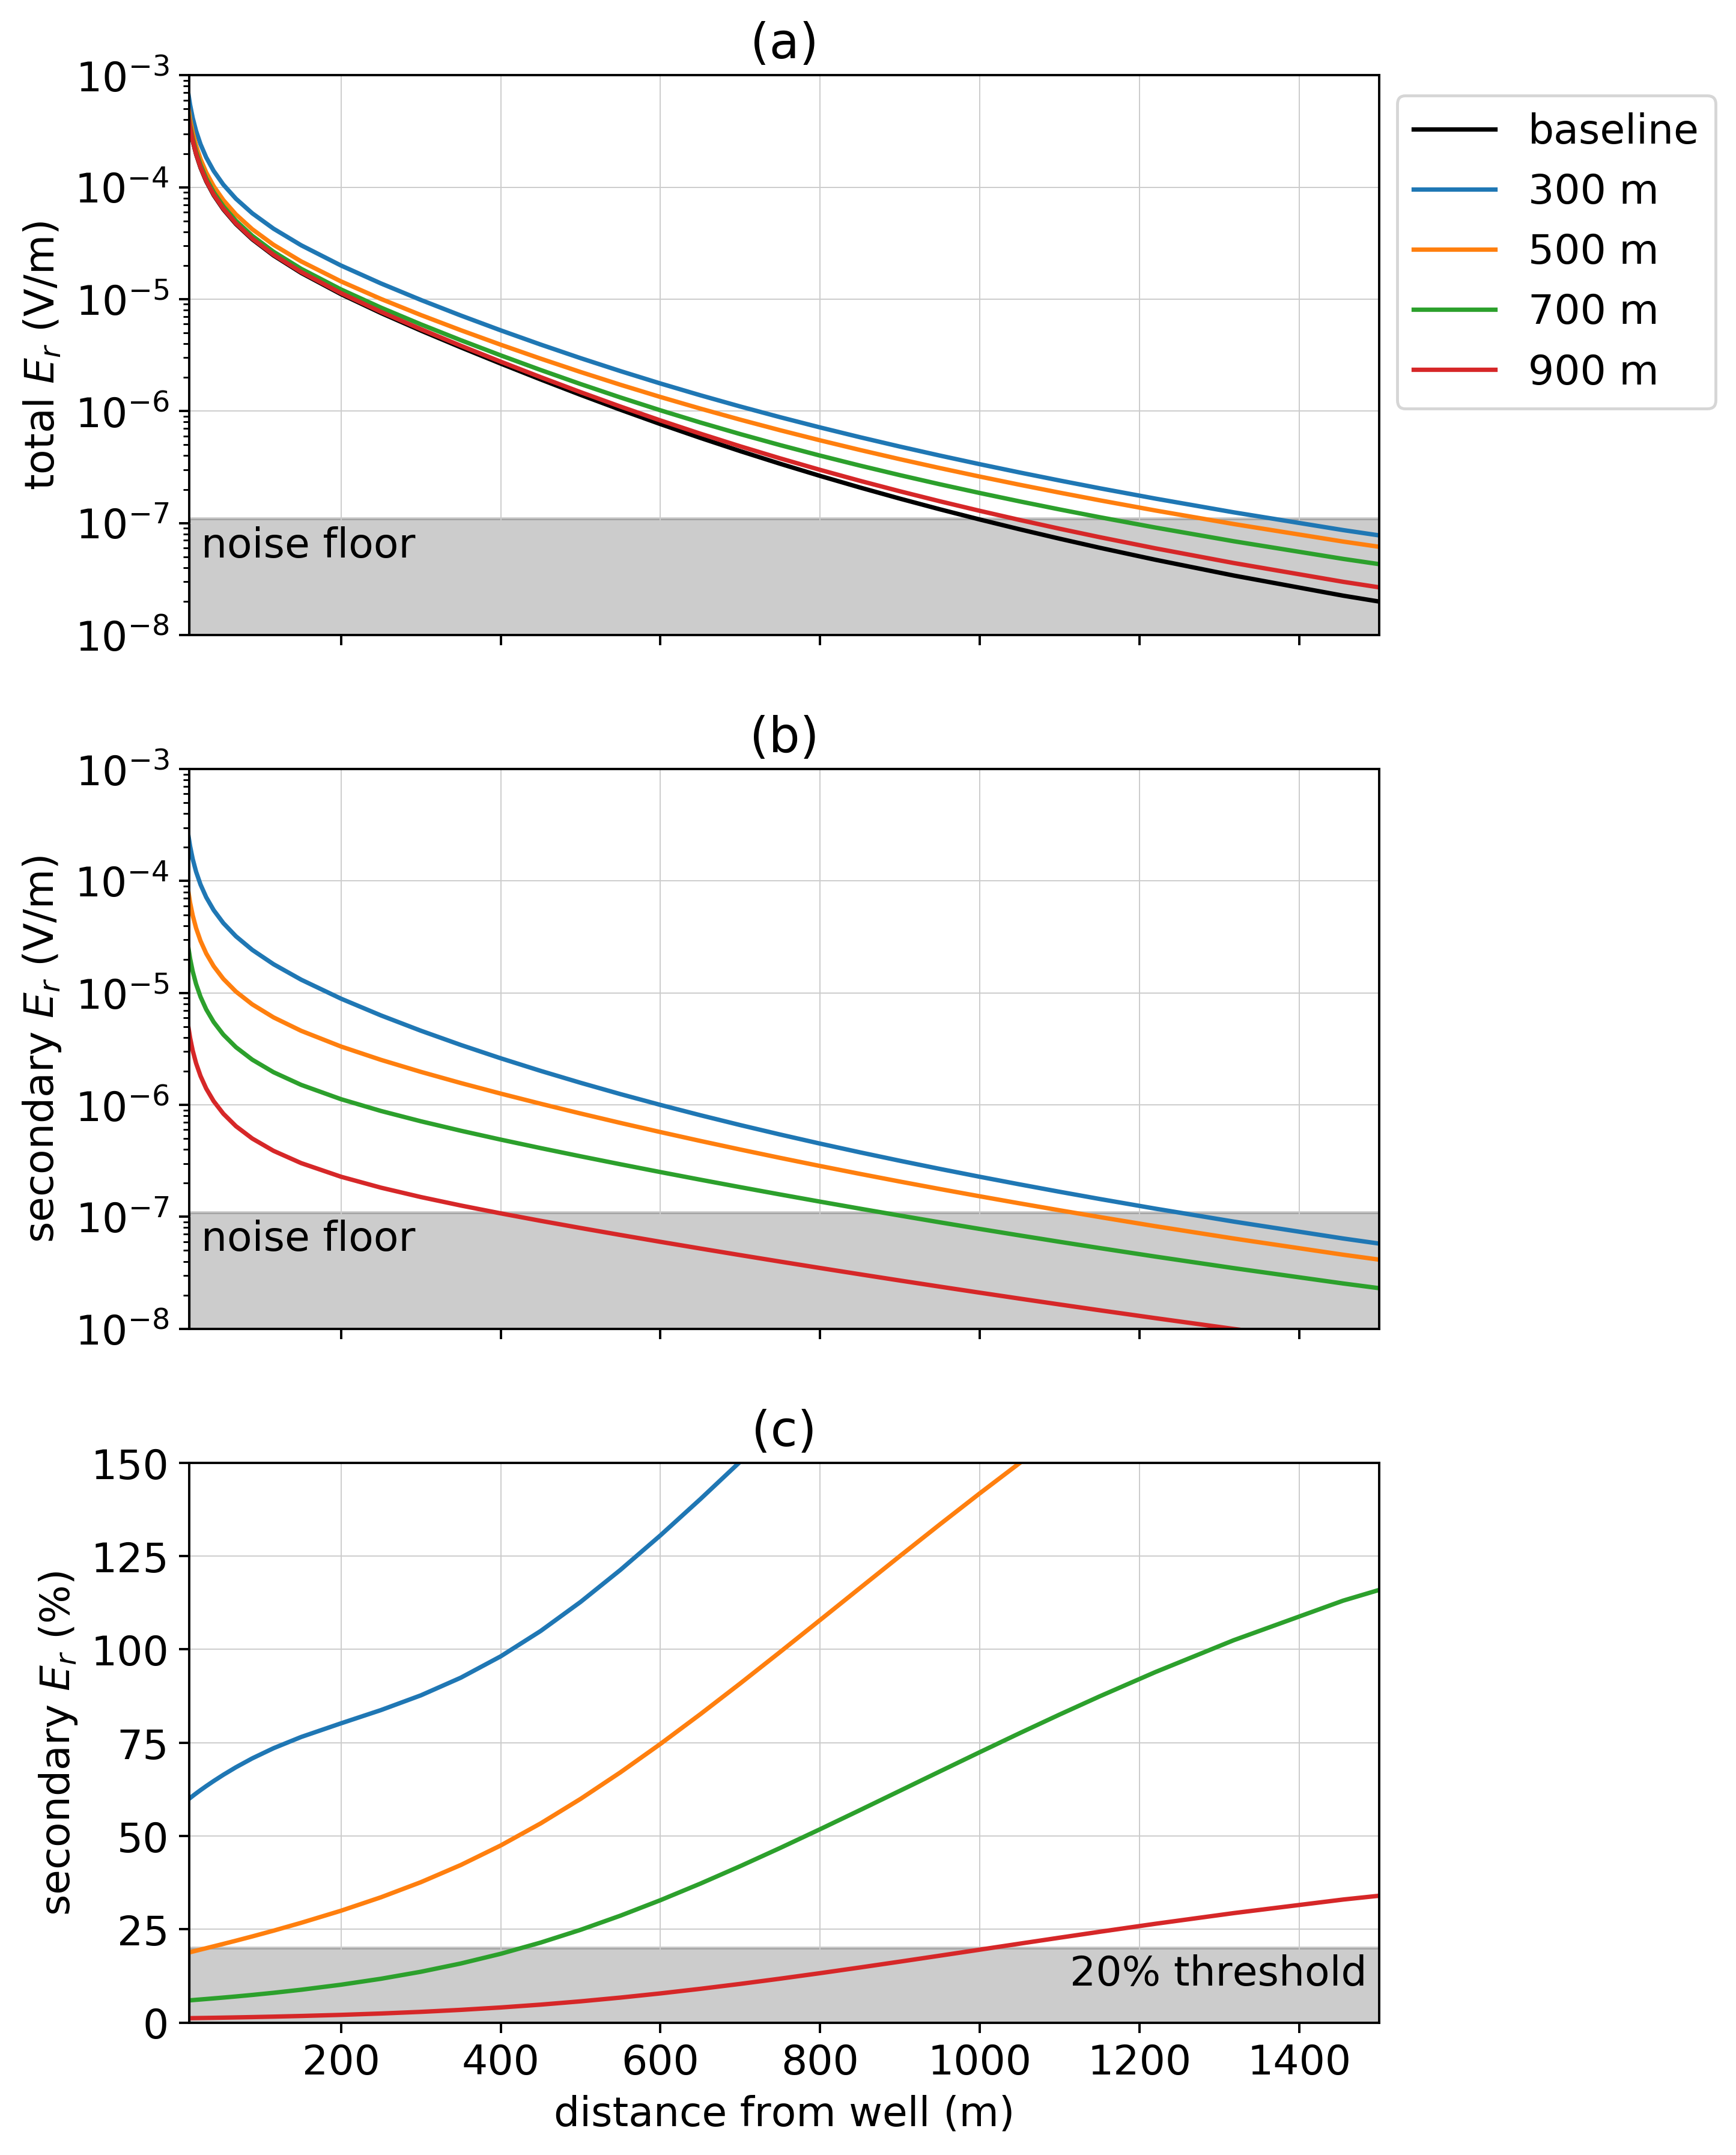
\includegraphics[width=0.8\textwidth]{figures/integrity_depth.png}
    \end{center}
\caption{
    Radial electric field as the depth of the flaw along a 1km long well is varied.
    The positive electrode is connected to the top of the casing, the negative electrode
    is positioned 500 m away and data are measured along a line $90^\circ$ from the
    source electrodes. In (a), we show the total electric field for four flawed wells,
    each with a 10 m flaw at the depth indicated on the legend. The black line shows
    the radial electric field due to an intact well; we define this as the primary.
    In (b), the secondary radial electric field is plotted and in (c), we show the
    secondary radial electric field as a percentage of the primary.
}
\label{fig:integrity_depth}
\end{figure}
